\documentclass[border=4pt]{standalone}
\usepackage{tikz}
\usetikzlibrary{arrows.meta,shapes.geometric}
\begin{document}
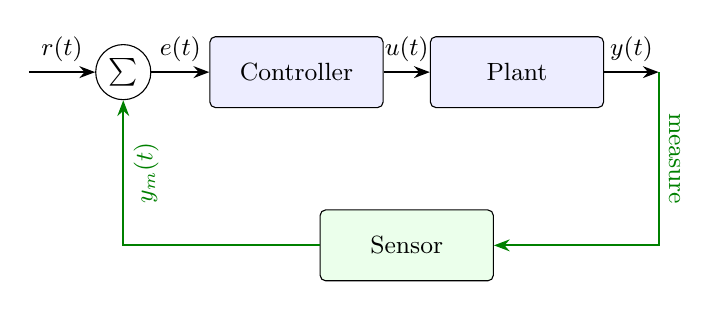
\begin{tikzpicture}[
  auto,
  block/.style={draw,rounded corners=2pt,minimum width=22mm,minimum height=9mm,fill=blue!7},
  signal/.style={-{Stealth[length=2mm]},thick},
  every node/.append style={font=\small}
]
  \coordinate (reference) at (0,0);
  \node[draw,circle,minimum size=7mm,inner sep=0pt] (sum) at (1.2,0) {$\sum$};
  \node[block] (controller) at (3.4,0) {Controller};
  \node[block] (plant) at (6.2,0) {Plant};
  \coordinate (output) at (8,0);
  \node[block,fill=green!8] (sensor) at (4.8,-2.2) {Sensor};

  \draw[signal] (reference) -- node[sloped] {$r(t)$} (sum);
  \draw[signal] (sum) -- node[sloped] {$e(t)$} (controller);
  \draw[signal] (controller) -- node[sloped] {$u(t)$} (plant);
  \draw[signal] (plant) -- node[sloped] {$y(t)$} (output);
  \draw[signal,green!50!black] (output) |- node[pos=.25,sloped] {measure} (sensor.east);
  \draw[signal,green!50!black] (sensor.west) -| node[pos=.75,sloped,swap] {$y_m(t)$} (sum.south);
\end{tikzpicture}
\end{document}
